\section{Graphical User Interface Design}
Designing the graphical interface began with simple mockups. A simple
initial diagram is shown below.

\begin{figure}[h]
    \frame{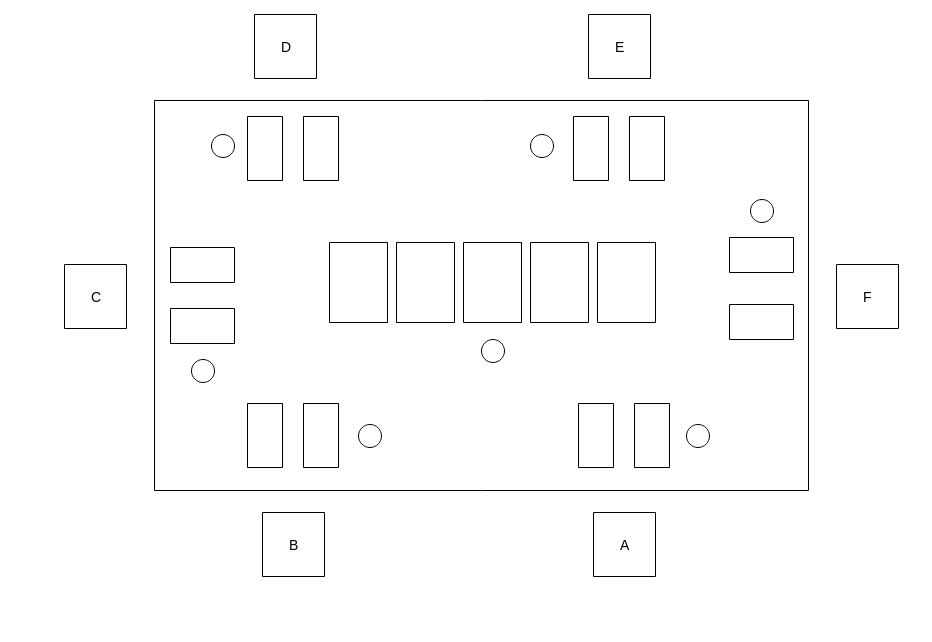
\includegraphics[width=\linewidth]{../images/initialgui.png}}
    \caption{Initial GUI mockup}%
    \label{fig:initialgui}
\end{figure}

This is a very standard design which cannot be varied much. All players have
two cards, a current bet, and a total amount of chips. As you may notice
in Figure~\ref{fig:initialgui} there is no label for the players total amount
of chips. This was instead decided to be stored as part of the name component,
as it makes for much less visual noise. The player labelled `A', is the
users player. He/she will always be seated here, and the other players will
be rotated around the board from their perspective. That is, every single
player A through F will appear to be in seat A from their own point of view.
Of course, this has been implemented to not affect how the gameplay works,
as the ordering of players is maintained, it is simply the visual
representation of the players which is being manipulated.

Of course, the players need some way to interact with the game, and simple
buttons which lie under the screen were used for this. The raise button
brought some complications, as the user has to enter a valid integer to
increase the current bet to. Some constraints are placed on this parameter.

\newpage

\begin{itemize}
\item The user must have enough chips to make the raise
\item The user must raise by at least the minimum raise
\item The raise must be an integer, not fractional
\end{itemize}

It was decided to use a separate window with a slider to handle the above
reasons. A slider has a minimum, and a maximum. This prevents the user from
both raising too little, and too much. And, by setting a slide interval, it
prevents the user selecting a non integer.

\begin{figure}[h]
    \centering
    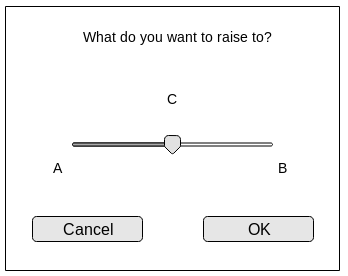
\includegraphics[width=0.5\linewidth]{../images/raisewindow.png}
    \caption{The Raise Window}%
    \label{fig:raisewindow}
\end{figure}

However, in the implementation of this, it was found that when displaying
the selected value, despite the steps being integer steps of one, 
fractional values could arise due to inherent errors in floating point 
mathematics. This was solved by simply taking the raw slider value, and 
casting it to an integer variable. This variable was then used for displaying 
the current users selection, and for the program to take as the chosen value 
once the `OK' button had been selected. Figure~\ref{fig:raisewindow} shows the 
raise window, where A is the minimum value, B is the maximum value, and C is 
the current value.

\begin{figure}
    \centering
    \begin{subfigure}[h]{0.4\textwidth}
        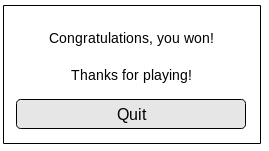
\includegraphics[width=\textwidth]{../images/winscreen.png}
        \caption{The Win Window}%
        \label{fig:winwindow}
    \end{subfigure}
    \begin{subfigure}[h]{0.4\textwidth}
        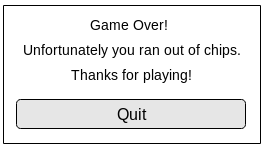
\includegraphics[width=\textwidth]{../images/lossscreen.png}
        \caption{The Loss Window}%
        \label{fig:losswindow}
    \end{subfigure}
    \caption{The Game Over Windows}\label{fig:gameoverwindows}
\end{figure}

Finally, there were elements needed for when a player either wins the game,
by the other players being eliminated for running out of chips, or when a
player loses, by being eliminated themselves. These took the form of simple
windows with configurable text, and a quit button. Both the win window
and the loss window use the same component, with only differing text. This
keeps the GUI consistent, and thus increases user acceptance.

Once the mockups had been completed the GUI was implemented in QtQML,
and hooked up to the Haskell code so it was fully usable and could be used
to test the poker game. Figure~\ref{fig:actualgui} shows the GUI in use,
with 6 players participating in a game. 

\begin{figure}[h]
    \centering
    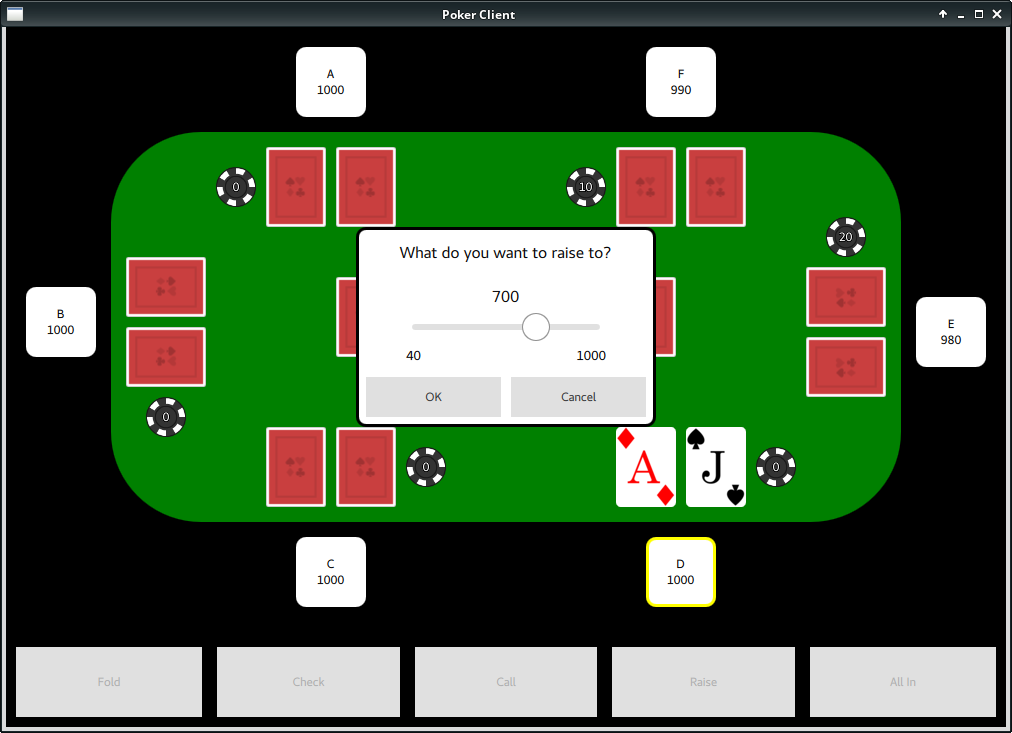
\includegraphics[width=\textwidth]{../images/actualgui.png}
    \caption{The initial implemented GUI}%
    \label{fig:actualgui}
\end{figure}

You can also see the implemented raise window in this image. Aside from the 
obvious card and poker chip assets, and colours, the implemented GUI is 
essentially the same as the mockup. One difference that was decided upon 
adding whilst testing, was a yellow border around the current player, so users 
would know how long it was until it was their turn. 

Another modification considered making was adding a dealer chip. Whilst
online poker does not have an actual player who deals the cards, and indeed
in real life poker the dealer is often not an actual player, the concept of
a dealer is still used.

Each round, the dealer progresses, and the player to
the left of the dealer is the player who bets first. In the preflop, this
player has to play a forced blind, but once in the flop and beyond, this player
gets to bet first, which is of some strategic importance. 

For these reasons, a dealer chip would seem obvious, however it was decided
against, because it both clutters the GUI, and the dealer can still be
recognised by simply observing who plays the small blind, and retaining this
information, knowing the dealer progresses once to the left each full round.
In the above screenshot for example, the dealer can be identified to be A,
as the player to his left has played a small blind of 10 chips.
